%\documentclass[a4paper]{article}
%\usepackage[T1]{fontenc}
%\usepackage[utf8]{inputenc}
%\usepackage[italian]{babel}
%\usepackage{amsmath}
%\usepackage{hyperref}
%\usepackage{amsthm}
%\usepackage{graphicx}
\documentclass[journal, a4paper]{IEEEtran}
\usepackage[italian]{babel}
\usepackage{booktabs}
\usepackage{siunitx}%Questo serve a caricare il pacchetto delle unità di misura del sistema internazionale%
\usepackage[utf8]{inputenc}
\usepackage{graphicx} 
\usepackage{url}
\usepackage{amsmath}
\usepackage{amssymb}
\usepackage{caption}
\usepackage{ textcomp }

\usepackage{keyval}
\usepackage{xcolor}
\usepackage{tikz}
\usepackage{circuitikz}
\usepackage{authblk}
%\usepackage{hyperref}

\begin{document}


% Define document title and author
	\title{Tecnologie Digitali - Relazione: convertitore di impedenza negativa e circuito Howland}
	\author[1]{Salvatore Bottaro}
		\author[2]{Lorenzo M. Perrone}
		\affil[1]{\texttt{salvo.bottaro@hotmail.it}}
		\affil[2]{\texttt{lorenzo.perrone.lmp@gmail.com}}
	\markboth{Tecnologie Digitali - Di Lieto}{}
	\maketitle

\begin{abstract}
In questa relazione mostriamo le caratteristiche e i limiti di un convertitore di impedenza negativa e la sua applicazione nel circuito Howland.
\end{abstract}

\section{Convertitore di impedenza negativa}
Si consideri il circuito in figura \ref{fig:negimp}.

\begin{figure}[htp]
\centering
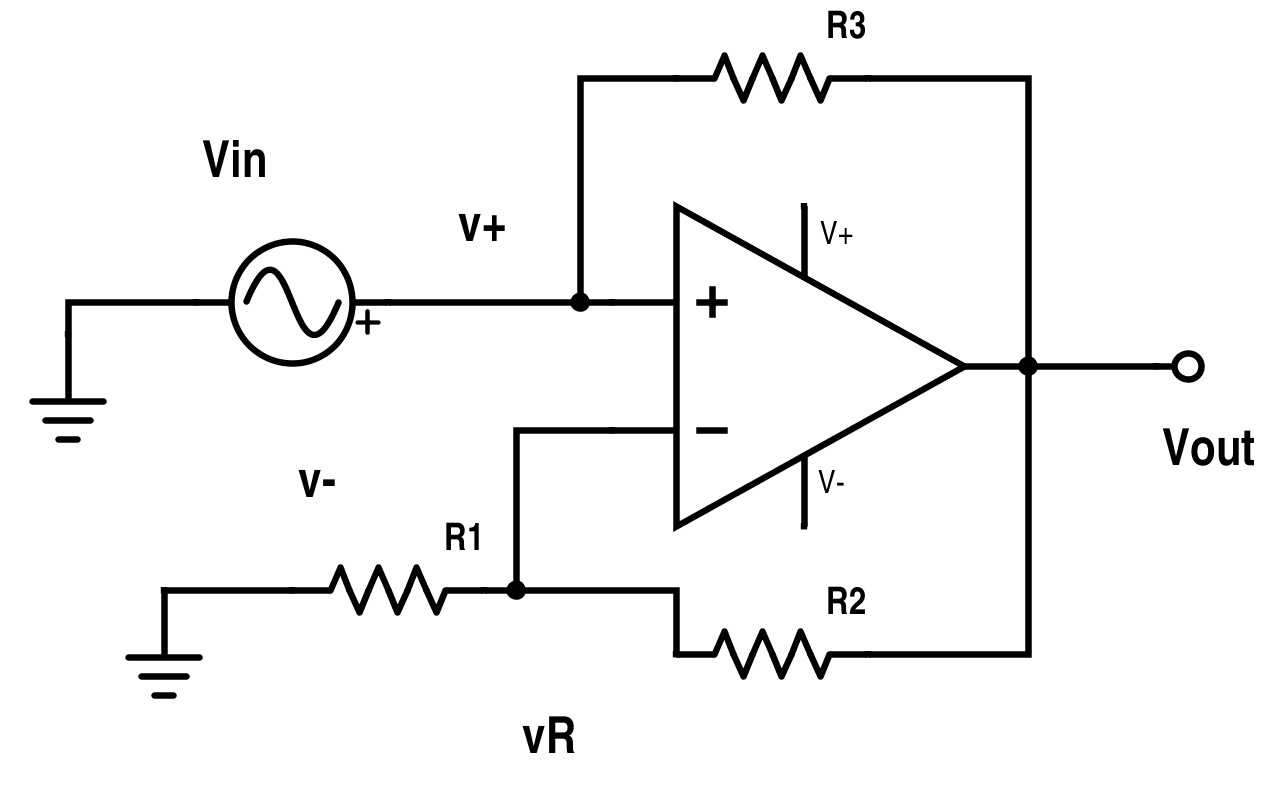
\includegraphics[scale=.2]{conv-imp-neg}
\caption{Convertitore di impedenza negativa}
\label{fig:negimp}
\end{figure}

Si mostri in che senso esso sia un convertitore di impedenza negativa applicando le regole d'oro dell'op-amp e risolvendo le equazioni del circuito. Come si vede in figura \ref{fig:negimp} la tensione $V_{In+}$ all'ingresso non-invertente dell'op-amp è la tensione $V_g$ del generatore VG. Per le regole d'oro dell'op-amp si ha la stessa tensione all'ingresso invertente ed essendo l'op-amp in configurazione non-invertente, tale tensione viene amplificata di un fattore $1+\frac{R_2}{R_1}$, da cui:
\begin{equation}
V_{out} = (1+\frac{R_2}{R_1})V_{in}
\label{eqn:amp}
\end{equation}

Pertanto la corrente che scorre da $V_{In+}$ a $V_{out}$ è data da:
\begin{equation}
I = \frac{V_{In+} - V_{out}}{R_3} = -\frac{R_2}{R_1 \, R_3}\, V_g \, \rightarrow V_g = -\frac{R_1\,R_3}{R_2}\,I
\end{equation}
da cui si evince come il generatore "veda" un'impedenza equivalente negativa.\\
Poiché l'espressione della resistenza equivalente segue direttamente dall'equazione \ref{eqn:amp} si ha che un modo per verificare il corretto comportamento del circuito è verificare se l'op-amp si comporta correttamente in configurazione non-invertente e dunque cercare di delineare i limiti di tale configurazione.\\
Per quanto riguarda il dimensionamento di $R_1$ e $R_2$ si ha che ovviamente esse devono essere tali che $V_{out}$ non sia troppo alto in rapporto alle tensioni di alimentazione. Come si legge dal foglio di specifiche, il \textit{Maximum peak output voltage swing} al massimo è $\pm 12$ \textdiv $14~V$, pertanto deve risultare:
\begin{equation}
V_{in}\,(1+\frac{R_2}{R_1}) \leq 12 \thicksim 14 V
\end{equation}
Ad esempio si confrontino le simulazioni fatte con TINA (vedi figura \ref{fig:negimpcon}) in cui sono stati impiegati Gain all'invertente G = 11 (figura \ref{fig:g_10_r_1k_dc_v})  G = 101 (figura \ref{g_100_r_1k_dc_v}). Si nota come nel primo caso il convertitore funzioni correttamente nel range di tensione scelto, nel secondo caso invece satura appena supera i 12 V.\\

\begin{figure}
\centering
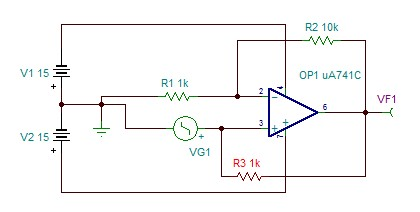
\includegraphics[scale=.6]{negatimpeconv}
\caption{Convertitore realizzato con TINA}
\label{fig:negimpcon}
\end{figure}

\begin{figure}[htp]
\centering
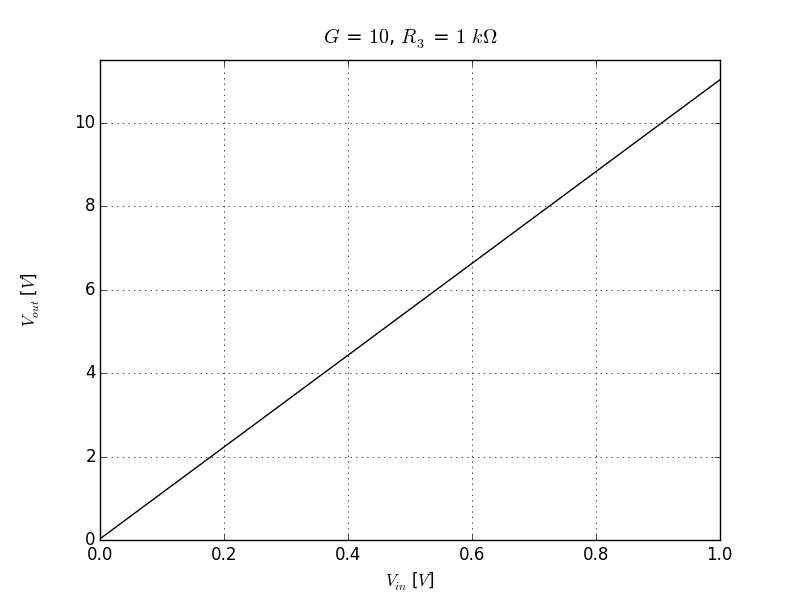
\includegraphics[scale=.35]{g_10_r_1k_dc_v}
\caption{Simulazione del convertitore per G=11}
\label{fig:g_10_r_1k_dc_v}
\end{figure}

\begin{figure}[htp]
\centering
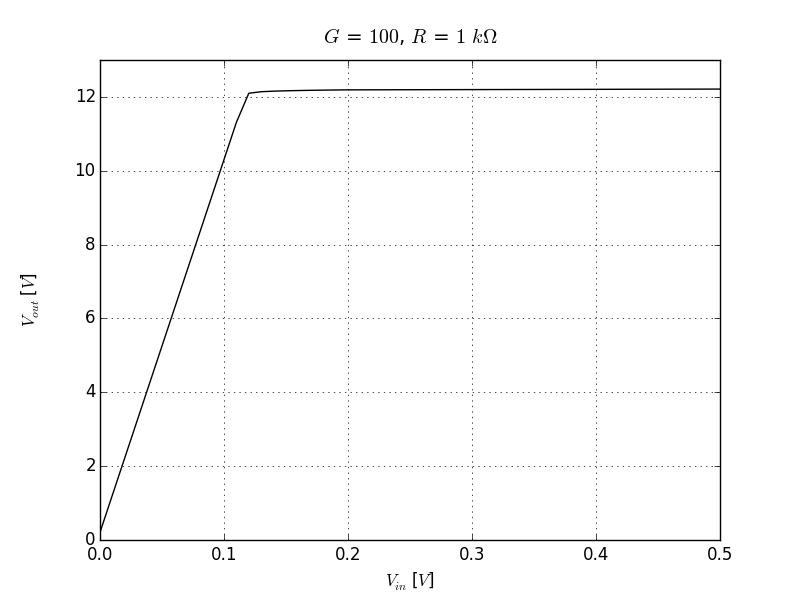
\includegraphics[scale=.35]{g_100_r_1k_dc_v}
\caption{Simulazione del convertitore con G=101}
\label{g_100_r_1k_dc_v}
\end{figure}

Per quanto riguarda $R_3$ invece, essa deve essere scelta in modo tale che non scorra troppa corrente verso il ramo non-invertente cosicché l'op-amp non riesca a stabilire il giusto feedback e dunque uguagliare le tensioni ai due ingressi, ovvero non deve essere troppo piccola. In figura \ref{g_10_r_300_dc_v} si vede come per tensioni vicine a 1 V si perda l'andamento lineare. 

\begin{figure}[htp]
\centering
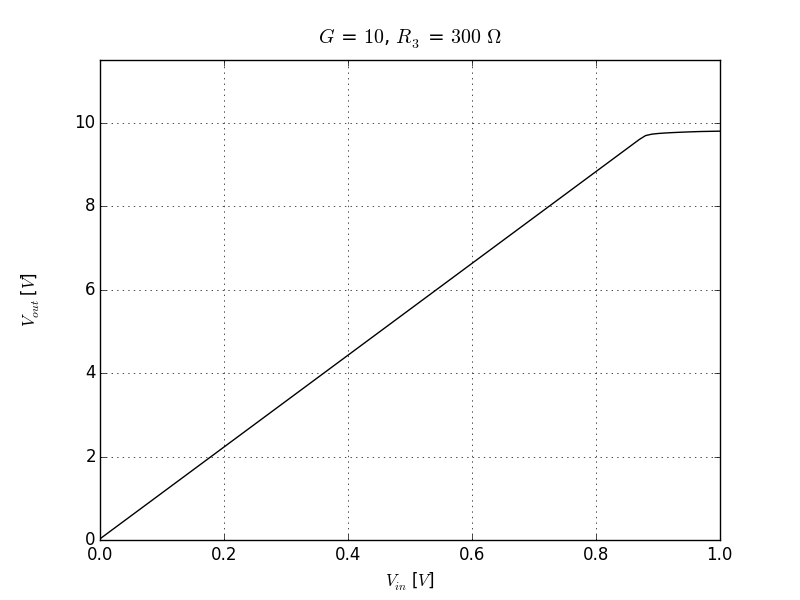
\includegraphics[scale=.35]{g_10_r_300_dc_v}
\caption{Simulazione del convertitore con G=11 e R=300 $\Omega$}
\label{g_10_r_300_dc_v}
\end{figure} 

Se si osserva il grafico in figura \ref{g_10_v_1_dc_r} si vede come per $V_{in} = 1 V$ il segnale in $V_{out}$ non dipenda da $R_3$ a partire dai 380 $\Omega$ circa.

\begin{figure}[htp]
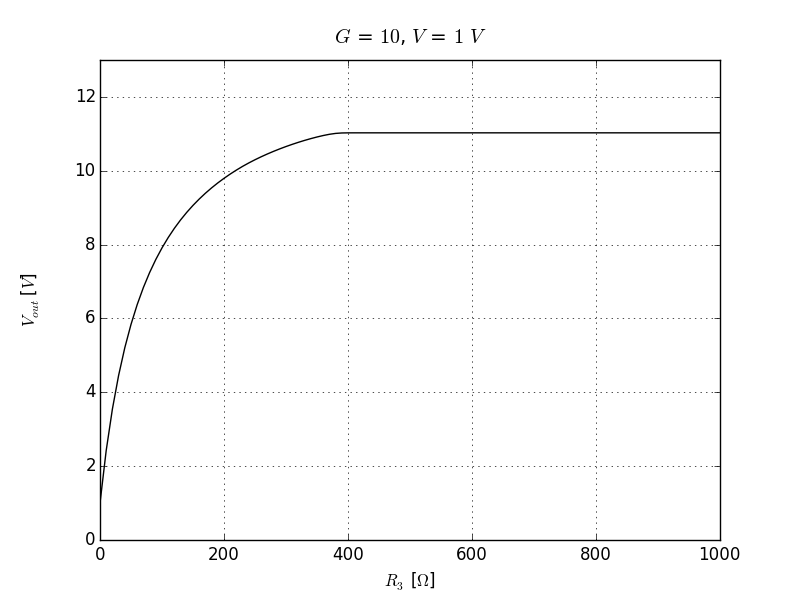
\includegraphics[scale=.4]{g_10_v_1_dc_r}
\caption{Dipendenza del segnale in uscita da $V_{out}$ in funzione di $R_3$ con G=11}
\label{g_10_v_1_dc_r} 
\end{figure}

Non disponendo di equazioni o modelli per dimensionare correttamente $R_3$, in base a varie prove effettuate possiamo fornire in tabella \ref{tab:r3} dei valori minimi indicativi per $R_3$ in funzione del gain G con una tensione di ingresso di 1 V.

\begin {table}[htp]
\caption {Valori minimi indicativi per $R_3$} 
\label{tab:r3} 
\begin{center}
\begin{tabular}{|c|c|}
\hline 
G & R \\ 
\hline 
11 & 380 \\ 
\hline 
10 & 230 \\ 
\hline 
9 & 150 \\ 
\hline 
8 & 110 \\ 
\hline 
7 & 80 \\ 
\hline 
6 & 60 \\ 
\hline 
\end{tabular} 
\end{center}
\end {table}

La possibilità di disporre di un circuito con impedenza equivalente negativa trova molte applicazioni, una di queste è il circuito di Howland.

\section{Circuito di Howland}

Lo schema del circuito di Howland è in figura \ref{fig:how}.

\begin{figure}[htp]
\centering
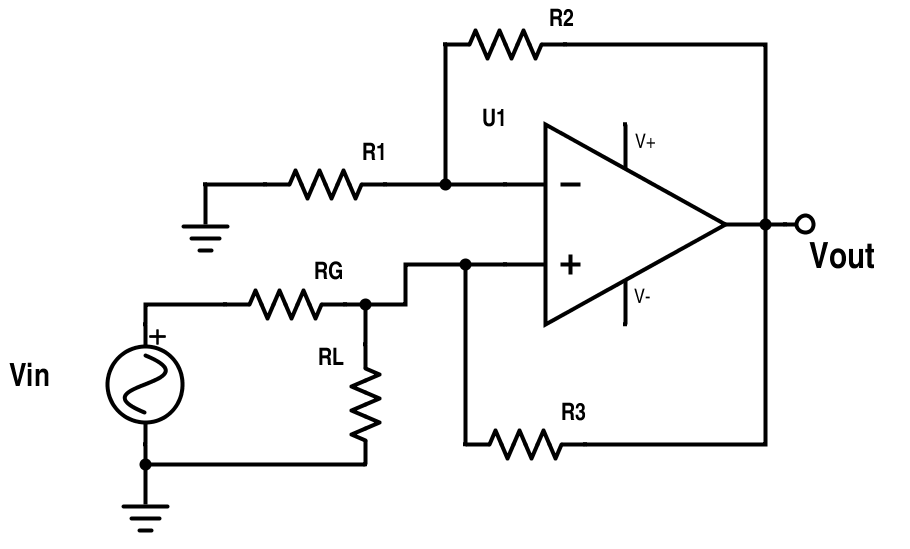
\includegraphics[scale=.3]{negative-impedance}
\caption{Circuito Howland}
\label{fig:how}
\end{figure}

In base ai risultati ottenuti in precedenza, il circuito è equivalente al parallelo fra le resistenze $R_G$, $R_L$ e $R_{eq}$ come si evince in figura \ref{fig:equiv}.

\begin{figure}[htp]
\centering
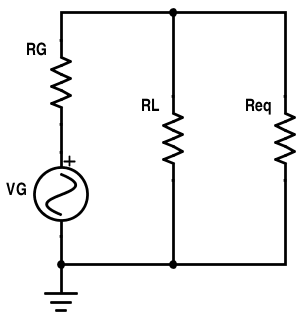
\includegraphics[scale=.4]{equivalent}
\caption{Circuito equivalente al circuito Howland}
\label{fig:equiv}
\end{figure}

Pertanto è immediato scrivere le equazioni che regolano il circuito. Prendendo come maglie fondamentali quella contenente il generatore e $R_L$ e quella contenente $R_L$ e $R_G$, e come verso convenzionale per le correnti $I_1$ e $I_2$ in entrambe le maglie quello antiorario, si hanno le seguenti equazioni:

\begin{equation}
V_G-R_G\,I_1-R_L\,I_1+R_L\,I_2 = 0
\end{equation}

\begin{equation}
-R_{eq}\,I_2+R_L\,I_1-R_L\,I_2 = 0
\end{equation}

Da cui si deducono le correnti:

\begin{equation}
I_1 = \frac{V_G(R_L + R_{eq})}{R_G\,R_L +R_L\,R_{eq} - R_G\,R_{eq}}
\end{equation}

\begin{equation}
I_2 = \frac{V_G\,R_L}{R_G\,R_L +R_L\,R_{eq} - R_G\,R_{eq}}
\end{equation}

Dal momento che la corrente che scorre in $R_L$ è $I_1 - I_2$, si ha, posto $R_{eq} = -R$:

\begin{equation}
I_L = I_1 - I_2 = - \frac{V_G\,R}{R_G\,R_L -R_L\,R + R_G\,R}
\end{equation}

Si vede come se nell'equazione precedente si pone $R_G=R$, l'espressione per $I_L$ diventa semplicemente:
\begin{equation}{\label{corr_carico}}
I_L = - \frac{V_G}{R}
\end{equation}

Ovvero la corrente che scorre nel carico $R_L$ non dipende dal carico, ovvero dimensionando opportunamente $R_1$, $R_2$ ed $R_3$ si  ha che il circuito Howland si comporta come un generatore ideale di corrente. Verifichiamo tramite delle simulazioni di TINA che questo comportamento sia rispettato, e in quali circostanze.\\
In Figura (\ref{fig:corrente_carico_res_carico_R3_500}) si riporta un grafico della corrente che attraversa la resistenza di carico $I_L$ in funzione della resistenza stessa $R_L$ in un intervallo 100 $\si{Ohm}$ - 100 $\si{kOhm}$, con resistenza del generatore arbitrariamente posta pari a $50 \si{Ohm}$, R1 = 1$\si{kOhm}$, R2 = 10$\si{kOhm}$, R3 = 500 $\si{Ohm}$.\\

\begin{figure}
\centering
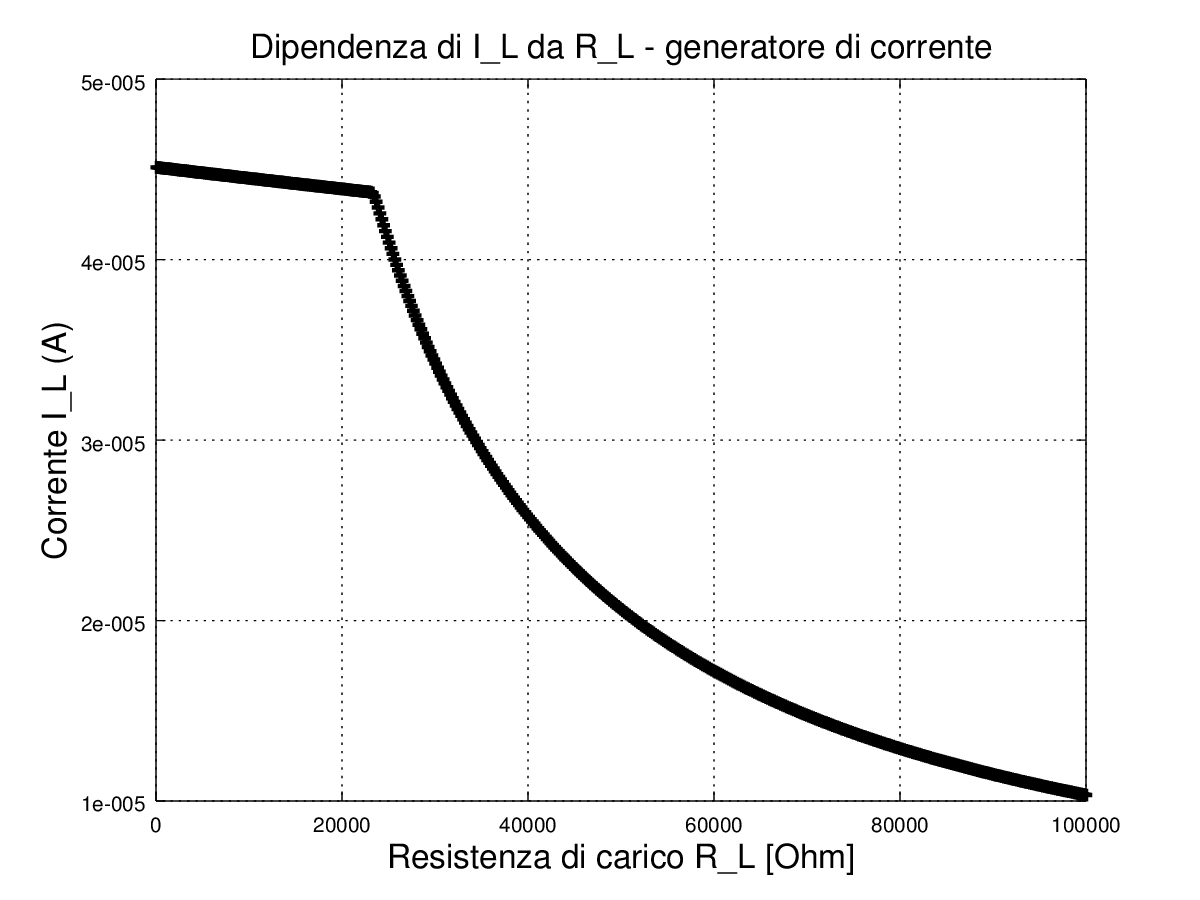
\includegraphics[width=0.7\linewidth]{./corrente_carico_res_carico_R3_500}
\caption{Plot della corrente $I_L$ su resistenza di carico $R_L$ per R3 = 500 Ohm, Vg = 0.5V, R2 = 10k, R1 = 1k, $R_g$ = 50 $\si{Ohm}$}
\label{fig:corrente_carico_res_carico_R3_500}
\end{figure}

Ciò che si nota immediatamente è che l'andamento della corrente si mantiene costante in una regione di \textit{plateau} nel range $R_L = $ 100-23k $\si{Ohm}$, nella quale ha un valore circa pari a $44 \pm 2 \mu \si{A}$, per poi decrescere sensibilmente tendendo a zero.\\
Ovviamente il nostro interesse si concentra sul comprendere quale è il motivo per cui si ha questo brusco cambiamento proprio al valore di $R_L$ di circa 23k$\si{Ohm}$ e, in un'ottica più concreta, come fare eventualmente ad estendere il \textit{plateau}.\\

Il primo tentativo effettuato è quello di raddoppiare la resistenza $R_3$ a 1k$\si{Ohm}$, e al tempo stesso raddoppiare $R_G$ a 100 $\si{Ohm}$ per far si che rimanga sempre valida la relazione $R = \frac{R_1 R_3 }{R_2}= R_G$. Il risultato è plottato in figura (\ref{fig:corrente_carico_res_carico_R3_500-1k_linear}), dove si vede il confronto con i valori precedenti.

\begin{figure}
\centering
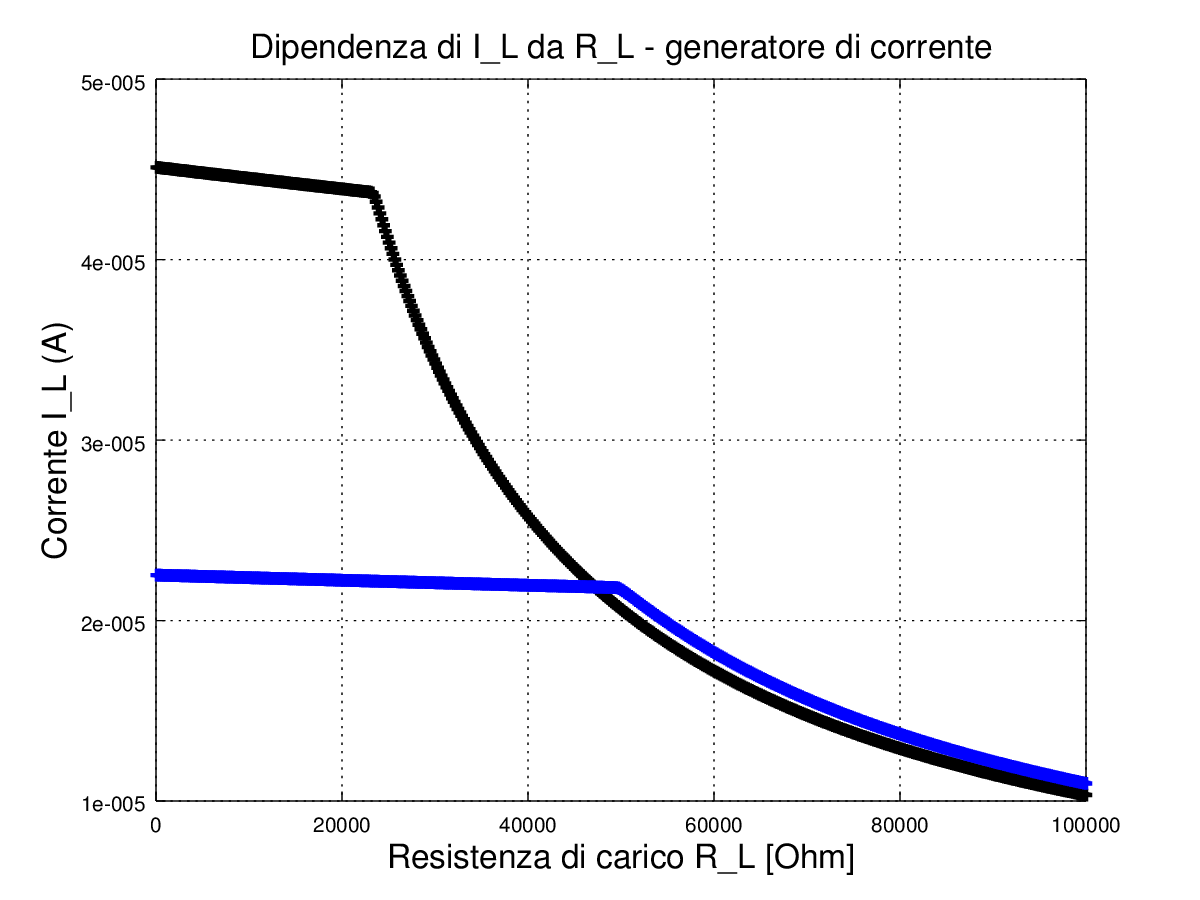
\includegraphics[width=0.7\linewidth]{./corrente_carico_res_carico_R3_500-1k_linear}
\caption{Plot della corrente $I_L$ su resistenza di carico $R_L$, per R3 = 500 Ohm (nero), e R3 = 1k (blu)}
\label{fig:corrente_carico_res_carico_R3_500-1k_linear}
\end{figure}


Come si può osservare, questa nuova scelta di resistenze ha esteso (raddoppiato) la zona di \textit{plateau}, fino al range di $R_L$ 100$\si{Ohm}$-52k $\si{Ohm}$. Continuando a raddoppiare $R_L$ e $R_G$ si verifica che il range (circa) raddoppia di estensione. I risultati di queste prove sono riportati in Figura (\ref{fig:corrente_carico_res_carico_R3_500-1k-2k-250_loglog}).

\begin{figure}
\centering
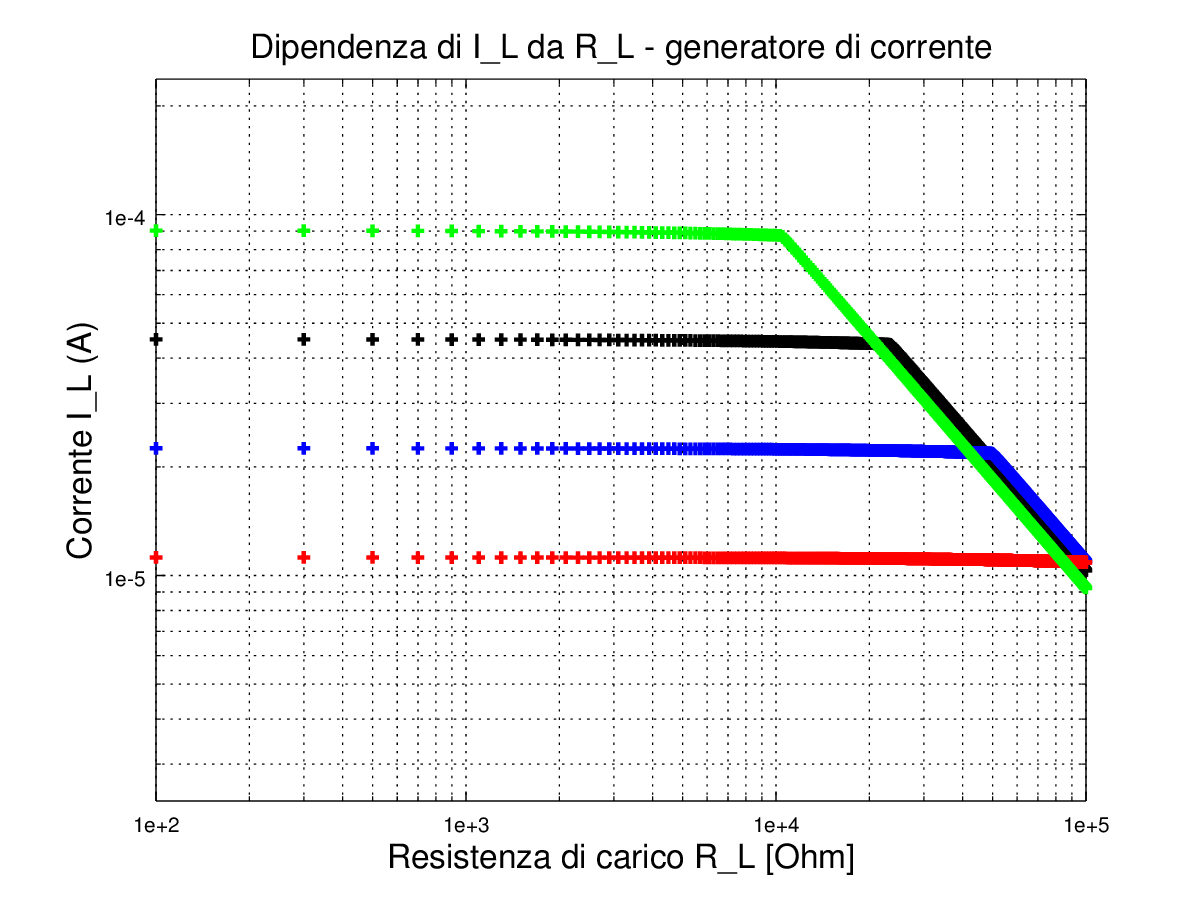
\includegraphics[width=0.7\linewidth]{./corrente_carico_res_carico_R3_500-1k-2k-250_loglog}
\caption{Dipendenza di $I_L$ da $R_L$ - raddoppiamo R3 e $R_G$: R3 = 250 (verde); R3 = 500 Ohm $R_G$ = 50 Ohm (nero); R3 = 1k $R_G$ = 100 Ohm (blu); R3 = 2k $R_G$ = 200 Ohm (rosso)}
\label{fig:corrente_carico_res_carico_R3_500-1k-2k-250_loglog}
\end{figure}

E' interessante notare come, sempre in base a quanto simulato da TINA, in questo modo si possa arrivare a rendere quasi del tutto costante il valore della corrente sul carico (di circa 1 $\mu$A) per un range di resistenze di quasi 4 ordini di grandezza, che fa capire piuttosto bene la definizione di "\textit{generatore ideale di corrente}" assegnata al circuito Howland.\\
Il passo successivo è cercare di mantenere costante il valore della resistenza del generatore $R_G$, che nella realtà è appunto un parametro fissato dal costruttore del generatore di tensione, e agire invece sui valori di $R_1$ e $R_3$. Ovviamente bisogna sempre far si che $R_G = \frac{R_1 R_3 }{R_2}$, quindi raddoppiando $R_3$ dimezzeremo $R_1$ e viceversa. Riportiamo una di queste simulazioni in Figura (\ref{fig:corrente_carico_res_carico_R3_125-250-500_R1-4k-2k-1k_linear1}), dove si vede che effettivamente il \textit{plateau} è aumentato, tuttavia in misura sensibilmente minore che nelle prove precedenti, oltre, ovviamente, a modificare il \textsc{gain} del circuito amplificante, che ricordiamo è pari a $G = 1 + \frac{R_2}{R_1}$.\\

\begin{figure}
\centering
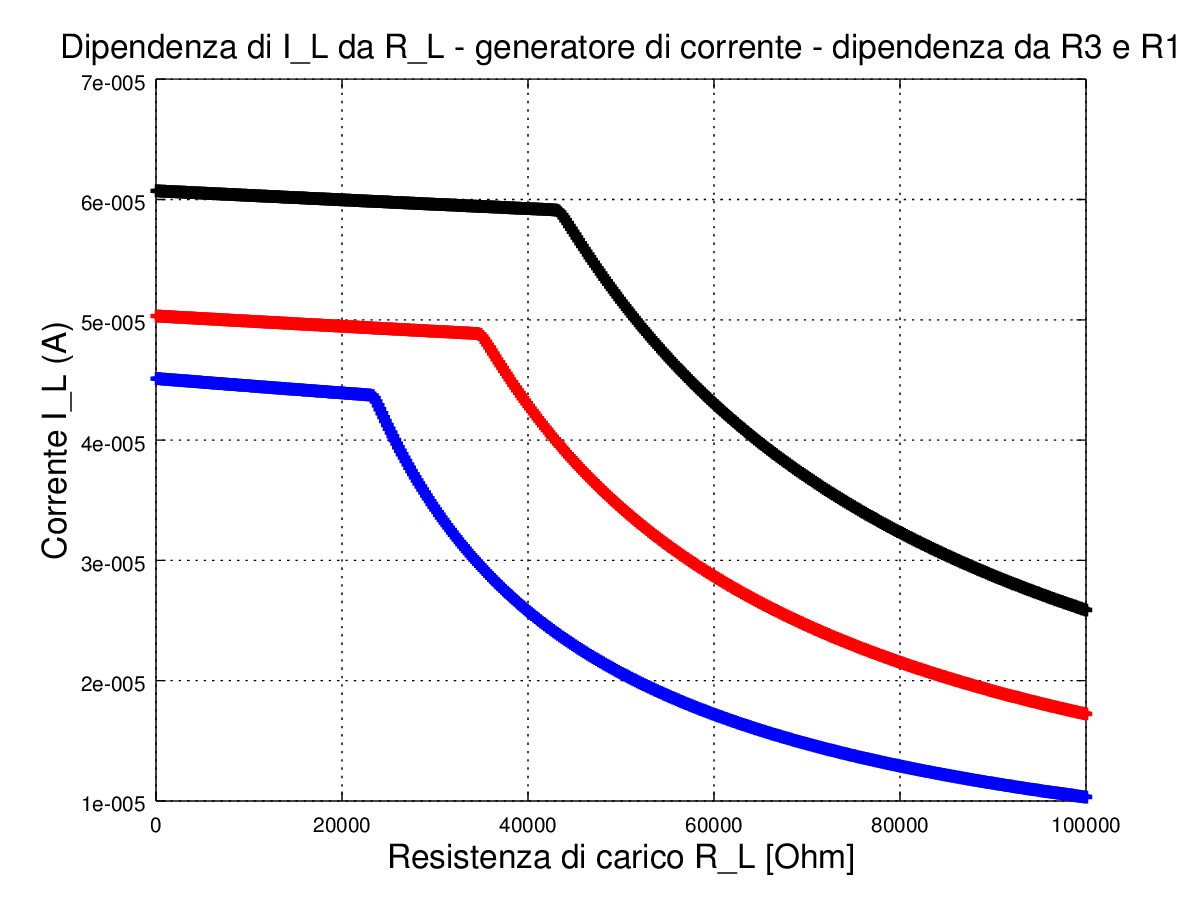
\includegraphics[width=0.7\linewidth]{./corrente_carico_res_carico_R3_125-250-500_R1-4k-2k-1k_linear1}
\caption{$I_L$ su $R_L$: dipendenza da R3 e R1 - raddoppiamo R3 e dimezziamo R1. R3 = 125Ohm, R1 = 4k (nero); R3 = 250 Ohm, R1 = 2k (rosso); R3 = 500 Ohm, R1 = 1k (blu)}
\label{fig:corrente_carico_res_carico_R3_125-250-500_R1-4k-2k-1k_linear1}
\end{figure}

\subsection{Relazione fra $V_{out}$ e $R_L$}

Rimane da capire quale potrebbe essere il motivo per cui il valore di $I_L$ smette di rimanere costante per decrescere rapidamente superata una certa soglia di $R_L$. Per far questo, procediamo con la risoluzione formale del circuito andando a ricavare la relazione fra la tensione di uscita dell'op-amp $V_{out}$ e $R_L$.\\

A partire dalla rappresentazione del circuito in Figura (\ref{fig:how}), è possibile scrivere con minima fatica le seguenti:

\begin{equation}
\begin{cases}
V_L = I_L \, R_L \\
V_{out} = (1+ \frac{R_2}{R_1})V_L
\end{cases}
\end{equation}

Da cui risulta:

\begin{equation}
V_{out} = I_L \, R_L (1+ \frac{R_2}{R_1})
\end{equation}

Dal momento che, come visto precedentemente, la corrente $I_L$ non dipende (o meglio, non dovrebbe dipendere) da $R_L$, a regime ci aspettiamo una proporzionalità di tipo lineare, con intercetta nulla e coefficiente angolare $ I_L \, (1+ \frac{R_2}{R_1})$. Verifichiamo questo andamento simulandolo con TINA, impiegando gli stessi valori di $R_3$, $R_G$ del grafico (\ref{fig:corrente_carico_res_carico_R3_500}). I risulati sono in Figura (\ref{fig:Vout_R_L_R3_500})

\begin{figure}
\centering
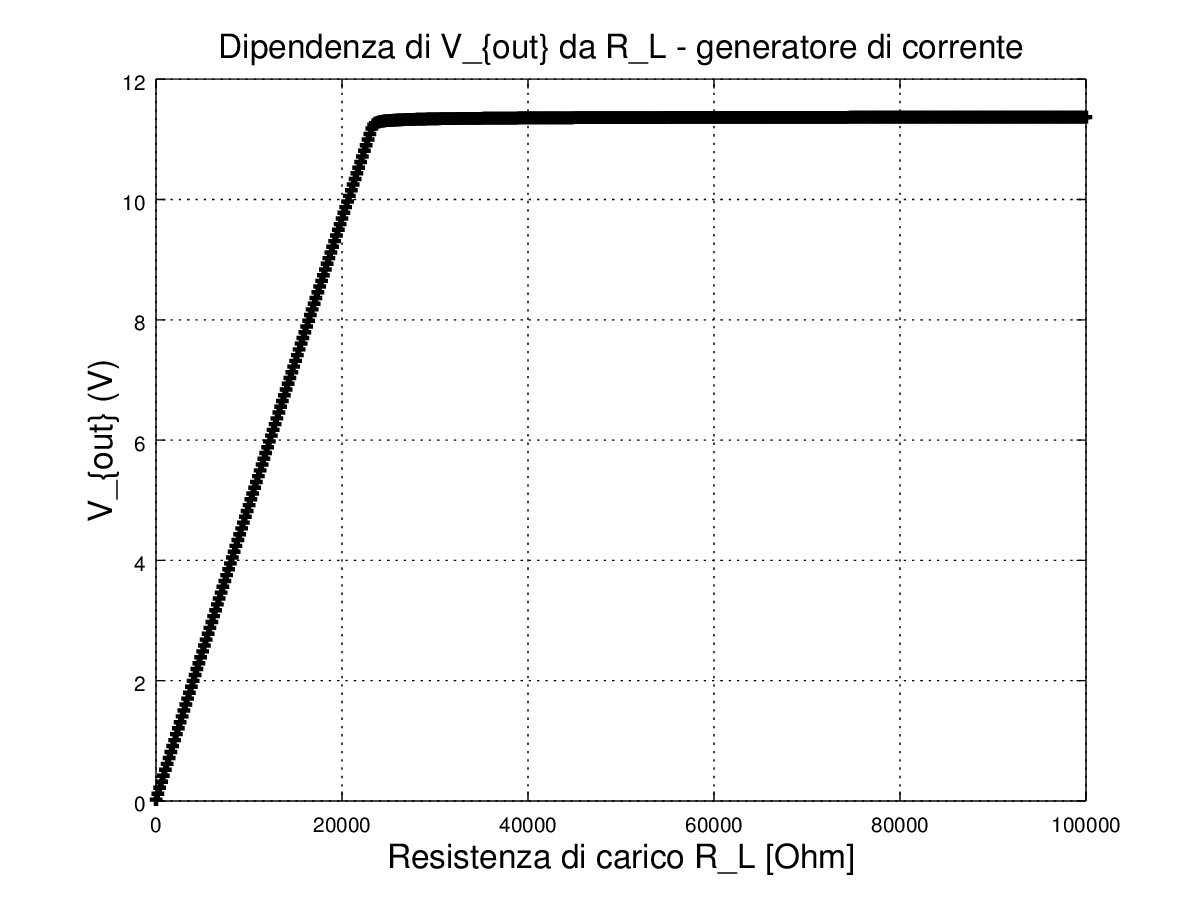
\includegraphics[width=0.7\linewidth]{./Vout_R_L_R3_500}
\caption{$V_{out}$ in funzione di $R_L$ a $R_3 = 500$ fissata, $V_G = 0.5V$}
\label{fig:Vout_R_L_R3_500}
\end{figure}

Dall'analisi di questo grafico seguono due importanti risultati:

\begin{itemize}
\item Capiamo finalmente per quale motivo per una resistenza di carico $R_L \gtrsim 20k\si{Ohm}$ la corrente $I_L$ termina il suo andamento costante. Infatti, come si può osservare, a tale resistenza coincide una tensione di output dell'op-amp di 11.3 V, subito in saturazione, per cui l'op-amp non riesce più a mantenere il \textit{feedback} sul ramo invertente, ed esce dal comportamento "ideale". Il valore $V_{out}$ di saturazione è strettamente correlato con la tensione di alimentazione $V_{CC}$ (che per queste simulazioni è stata posta a $\pm 15$ V), e infatti all'aumentare di quest'ultima si verifica un incremento della regione di \textit{plateau}.

\item L'andamento lineare è molto ben rispettato e una stima del coefficiente angolare della retta, pari a $m_{meas} \simeq 4.8 \, 10^{-4} \, \si{V/ Ohm}$ risulta essere in accordo con quello aspettato, calcolato moltiplicando il valore "costante" della corrente quando $R_L \leq 20k\si{Ohm}$ per il gain $G = 1 + \frac{R_2}{R_1} \simeq 11$ del circuito, da cui risulta che $ m_{exp} \simeq 4.8 \, 10^{-4} \si{V/ Ohm}$.\\
\end{itemize} 

\textsc{PROBLEMA!}
Tuttavia, proprio quest'ultimo risultato ci pone davanti ad un'incongruenza con le relazioni ricavate nella prima parte della relazione. Infatti, nella (\ref{corr_carico}) si è visto che $I_L = - \frac{V_G}{R}$ che, per i valori impiegati nell'ultima simulazione, e cioè $R = R_g$ = 50 $\si{Ohm}$ e $V_G = 0.5V$, implica una corrente $I_L$ dell'ordine della decina di mA, e non decina di $\mu$A, come ricavato dalle simulazioni precedenti. Riteniamo che ci possa essere un errore, o una ipotesi non del tutto verificata nella risoluzione del circuito, che dia origine a questa evidente discrepanza, che nonostante gli sforzi non siamo riusciti a localizzare.


A questo punto, avendo analizzato approfonditamente il comportamento simulato del circuito, e identificato un range per alcuni parametri tipici in cui il circuito di Howlen sembra funzionare, abbiamo montato sulla \textit{breadboard} i componenti, tra cui un potenziometro variabile fra $108-1020 \pm 1\% \si{Ohm}$ che avrebbe giocato il ruolo di carico $R_L$. Con nostro grandissimo dispiacere non siamo riusciti ad ottenere alcuna serie di misure "utili" con il VI di acquisizione, nonostante vari tentativi. E' utile riportare di seguito i valori delle resistenze e alcune osservazioni.\\
 
{ 
\centering

\begin{tabular}{|c|c|}
\hline \textbf{Resistenze} & \textbf{Valori} \\ 
\hline R1 & 1  k$\si{Ohm}$ $\pm 5\%$\\ 
\hline R2 & 10  k$\si{Ohm}$ $\pm 5\%$ \\ 
\hline R3 & 10k$\si{Ohm}$ $\pm 5\%$\\ 
\hline $R_G$ & 100$\si{Ohm}$ $\pm 5\%$\\ 
\hline $R_L$ & 108-1210 $\pm 1\% \si{Ohm}$ \\ 
\hline 
\end{tabular}

}


\section{Osservazioni}

\begin{itemize}
\item Le resistenze sono state dimensionate in modo da rimanere nel "range di validità" del modello, come ricavato nelle simulazioni;

\item La resistenza del generatore $R_G$ è stata arbitrariamente scelta da noi, con un valore abbastanza sensato (100 $\si{Ohm}$), e collegata in serie al generatore stesso;

\item La tensione fornita dal generatore di tensione appositamente impiegato per questa esperienza (e non l'\textsc{atten} usuale) è circa di 1 V, per cui, a partire dalla $I_L = - \frac{V_G}{R_G}$, ci aspettiamo una corrente nel circuito di carico di 10 mA, al di sotto del valore tipico per l'op-amp \textsc{$\mu$ A741cp} che è di 25 mA, con un massimo dichiarato di 40 mA;

\item Il primo segnale acquisito dal VI, la tensione in uscita dall'op-amp $V_{out}$ era del tutto saturato impiegando un fondoscala a 10 V. Il gain previsto era circa 11, per cui abbiamo esplorato valori di $V_{in}$ intorno a mezzo volt, tuttavia abbiamo continuato a non osservare altro che la saturazione a +10V.

\item Per comprendere meglio cosa non stesse funzionando secondo le aspettative, è stato posto un multimetro digitale in modalità amperometro in serie al carico. Il valore di corrente aspettato doveva essere maggiore di 10mA (20, 30 in base al $V_{in}$ impostato), ma l'amperometro non ha mai registrato un valore superiore a circa 6mA.

\item Una prima, e probabilmente fondata ipotesi, è che nel circuito in esame parte della corrente prodotta dall'op-amp venisse immessa dentro il generatore, e che quindi ciò modificasse il comportamento dell'Howland.

\item Per verificare questa supposizione abbiamo scollegato il generatore di tensione in uso per impiegare la boccola a 5V dell'\textsc{atten}, costruendo un partitore di tensione 1:10 in modo da fornire come $V_{in}$ sul ramo non invertente circa 0.5V. La cosa che ci ha sorpreso più di tutto è che pur avendo montato il partitore, misurando con un secondo multimetro la tensione in ingresso, questa rimanesse comunque a circa 5V. Il buon funzionamento del partitore è stato verificato scollegando l'op-amp, e la tensione letta era circa 0.5V, come aspettato, ma ricollegando nuovamente il partitore al circuito, il valore tornava a 5V. 

\item L'unica conclusione che abbiamo potuto trarre è che l'inserimento di un generatore di tensione perturbava enormemente il comportamento modellizzato del circuito di Howland, e in particolare tale perturbazione si potrebbe ascrivere alla corrente che dal circuito rientra nel generatore. Una verifica sensata consisterebbe nel provare a collegare una pila al posto del generatore, poichè quest'ultima non dovrebbe essere influenzata dal resto del circuito.

\item Come ultima osservazione, è da rilevare che, anche nelle simulazioni di TINA, anche una differenza di qualche decina di $\Omega$ fra $R_G$ e $R_{eq}$, che devono essere uguali per evidenziare il comportamente di \textit{Negative Impedance Converter}, era sufficiente per modificare drasticamente l'andamento della corrente $I_L$ in funzione della resistenza di carico $R_L$. Dal momento che la nostra $R_G$ era collegata in serie al generatore, la sua resistenza "reale" interna, sommata a $R_G$, potrebbe essere risultata sensibilmente diversa dalla nostra $R_{eq}$, e quindi aver contribuito al cattivo funzionamento del circuito.

\end{itemize}
\begin{thebibliography}{5}

	%Each item starts with a \bibitem{reference} command and the details thereafter.
	\bibitem{HOP96} % Transaction paper
	Datasheet, $\mu $A741 General-Purpose Operational Amplifiers. SLOS094E – NOVEMBER 1970  –REVISED JANUARY 2015.
	\url{http://www.ti.com/lit/ds/symlink/ua741.pdf}


	\bibitem{M06} % Conference paper
	Paul Horowitz, Winfield Hill - The Art of Electronics. Cambridge University Press (1989).
	
\end{thebibliography}

% Your document ends here!
\end{document}
